\documentclass[1p]{elsarticle_modified}
%\bibliographystyle{elsarticle-num}

%\usepackage[colorlinks]{hyperref}
%\usepackage{abbrmath_seonhwa} %\Abb, \Ascr, \Acal ,\Abf, \Afrak
\usepackage{amsfonts}
\usepackage{amssymb}
\usepackage{amsmath}
\usepackage{amsthm}
\usepackage{scalefnt}
\usepackage{amsbsy}
\usepackage{kotex}
\usepackage{caption}
\usepackage{subfig}
\usepackage{color}
\usepackage{graphicx}
\usepackage{xcolor} %% white, black, red, green, blue, cyan, magenta, yellow
\usepackage{float}
\usepackage{setspace}
\usepackage{hyperref}

\usepackage{tikz}
\usetikzlibrary{arrows}

\usepackage{multirow}
\usepackage{array} % fixed length table
\usepackage{hhline}

%%%%%%%%%%%%%%%%%%%%%
\makeatletter
\renewcommand*\env@matrix[1][\arraystretch]{%
	\edef\arraystretch{#1}%
	\hskip -\arraycolsep
	\let\@ifnextchar\new@ifnextchar
	\array{*\c@MaxMatrixCols c}}
\makeatother %https://tex.stackexchange.com/questions/14071/how-can-i-increase-the-line-spacing-in-a-matrix
%%%%%%%%%%%%%%%

\usepackage[normalem]{ulem}

\newcommand{\msout}[1]{\ifmmode\text{\sout{\ensuremath{#1}}}\else\sout{#1}\fi}
%SOURCE: \msout is \stkout macro in https://tex.stackexchange.com/questions/20609/strikeout-in-math-mode

\newcommand{\cancel}[1]{
	\ifmmode
	{\color{red}\msout{#1}}
	\else
	{\color{red}\sout{#1}}
	\fi
}

\newcommand{\add}[1]{
	{\color{blue}\uwave{#1}}
}

\newcommand{\replace}[2]{
	\ifmmode
	{\color{red}\msout{#1}}{\color{blue}\uwave{#2}}
	\else
	{\color{red}\sout{#1}}{\color{blue}\uwave{#2}}
	\fi
}

\newcommand{\Sol}{\mathcal{S}} %segment
\newcommand{\D}{D} %diagram
\newcommand{\A}{\mathcal{A}} %arc


%%%%%%%%%%%%%%%%%%%%%%%%%%%%%5 test

\def\sl{\operatorname{\textup{SL}}(2,\Cbb)}
\def\psl{\operatorname{\textup{PSL}}(2,\Cbb)}
\def\quan{\mkern 1mu \triangleright \mkern 1mu}

\theoremstyle{definition}
\newtheorem{thm}{Theorem}[section]
\newtheorem{prop}[thm]{Proposition}
\newtheorem{lem}[thm]{Lemma}
\newtheorem{ques}[thm]{Question}
\newtheorem{cor}[thm]{Corollary}
\newtheorem{defn}[thm]{Definition}
\newtheorem{exam}[thm]{Example}
\newtheorem{rmk}[thm]{Remark}
\newtheorem{alg}[thm]{Algorithm}

\newcommand{\I}{\sqrt{-1}}
\begin{document}

%\begin{frontmatter}
%
%\title{Boundary parabolic representations of knots up to 8 crossings}
%
%%% Group authors per affiliation:
%\author{Yunhi Cho} 
%\address{Department of Mathematics, University of Seoul, Seoul, Korea}
%\ead{yhcho@uos.ac.kr}
%
%
%\author{Seonhwa Kim} %\fnref{s_kim}}
%\address{Center for Geometry and Physics, Institute for Basic Science, Pohang, 37673, Korea}
%\ead{ryeona17@ibs.re.kr}
%
%\author{Hyuk Kim}
%\address{Department of Mathematical Sciences, Seoul National University, Seoul 08826, Korea}
%\ead{hyukkim@snu.ac.kr}
%
%\author{Seokbeom Yoon}
%\address{Department of Mathematical Sciences, Seoul National University, Seoul, 08826,  Korea}
%\ead{sbyoon15@snu.ac.kr}
%
%\begin{abstract}
%We find all boundary parabolic representation of knots up to 8 crossings.
%
%\end{abstract}
%\begin{keyword}
%    \MSC[2010] 57M25 
%\end{keyword}
%
%\end{frontmatter}

%\linenumbers
%\tableofcontents
%
\newcommand\colored[1]{\textcolor{white}{\rule[-0.35ex]{0.8em}{1.4ex}}\kern-0.8em\color{red} #1}%
%\newcommand\colored[1]{\textcolor{white}{ #1}\kern-2.17ex	\textcolor{white}{ #1}\kern-1.81ex	\textcolor{white}{ #1}\kern-2.15ex\color{red}#1	}

{\Large $\underline{12a_{0083}~(K12a_{0083})}$}

\setlength{\tabcolsep}{10pt}
\renewcommand{\arraystretch}{1.6}
\vspace{1cm}\begin{tabular}{m{100pt}>{\centering\arraybackslash}m{274pt}}
\multirow{5}{120pt}{
	\centering
	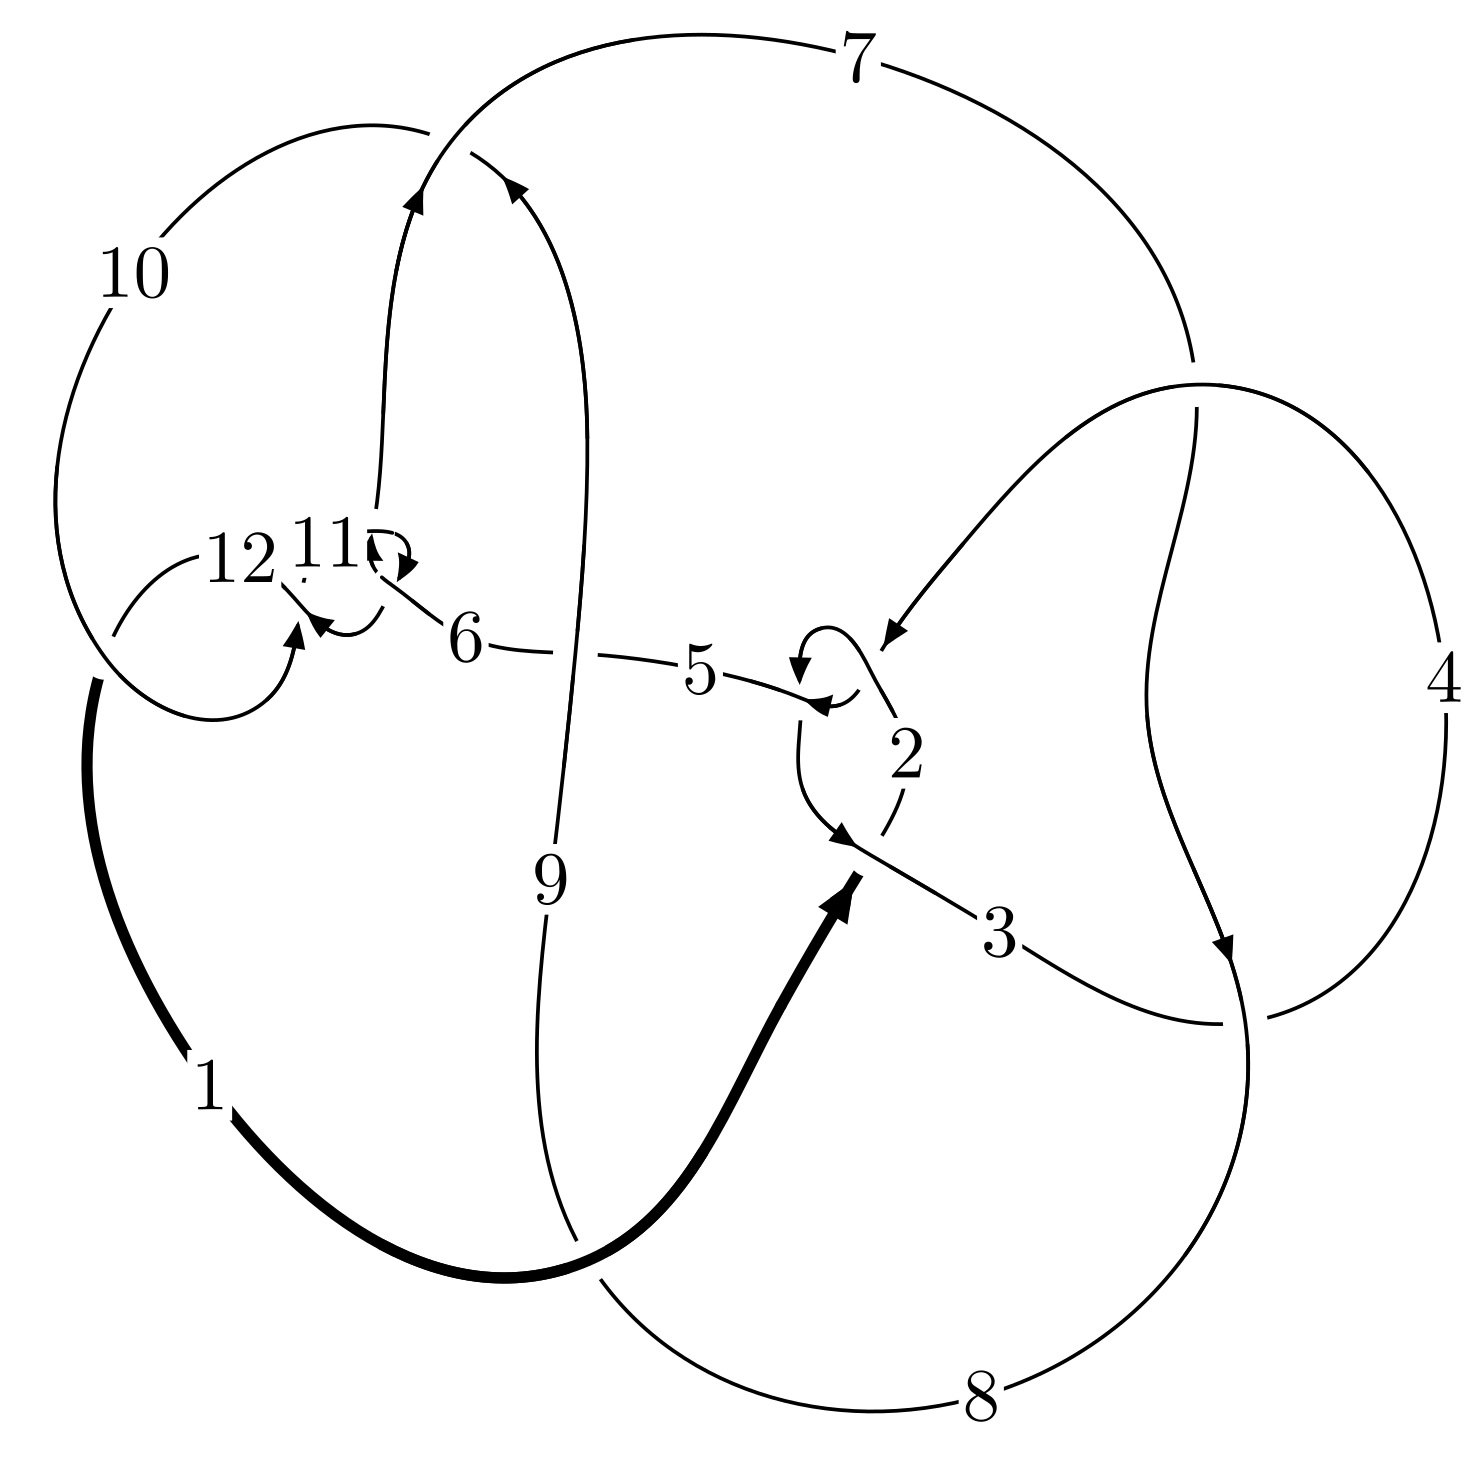
\includegraphics[width=112pt]{../../../GIT/diagram.site/Diagrams/png/884_12a_0083.png}\\
\ \ \ A knot diagram\footnotemark}&
\allowdisplaybreaks
\textbf{Linearized knot diagam} \\
\cline{2-2}
 &
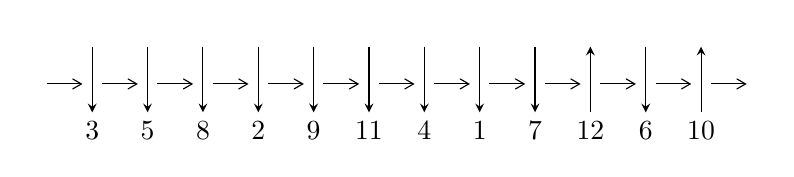
\begin{tikzpicture}[x=20pt, y=17pt]
	% nodes
	\node (C0) at (0, 0) {};
	\node (C1) at (1, 0) {};
	\node (C1U) at (1, +1) {};
	\node (C1D) at (1, -1) {3};

	\node (C2) at (2, 0) {};
	\node (C2U) at (2, +1) {};
	\node (C2D) at (2, -1) {5};

	\node (C3) at (3, 0) {};
	\node (C3U) at (3, +1) {};
	\node (C3D) at (3, -1) {8};

	\node (C4) at (4, 0) {};
	\node (C4U) at (4, +1) {};
	\node (C4D) at (4, -1) {2};

	\node (C5) at (5, 0) {};
	\node (C5U) at (5, +1) {};
	\node (C5D) at (5, -1) {9};

	\node (C6) at (6, 0) {};
	\node (C6U) at (6, +1) {};
	\node (C6D) at (6, -1) {11};

	\node (C7) at (7, 0) {};
	\node (C7U) at (7, +1) {};
	\node (C7D) at (7, -1) {4};

	\node (C8) at (8, 0) {};
	\node (C8U) at (8, +1) {};
	\node (C8D) at (8, -1) {1};

	\node (C9) at (9, 0) {};
	\node (C9U) at (9, +1) {};
	\node (C9D) at (9, -1) {7};

	\node (C10) at (10, 0) {};
	\node (C10U) at (10, +1) {};
	\node (C10D) at (10, -1) {12};

	\node (C11) at (11, 0) {};
	\node (C11U) at (11, +1) {};
	\node (C11D) at (11, -1) {6};

	\node (C12) at (12, 0) {};
	\node (C12U) at (12, +1) {};
	\node (C12D) at (12, -1) {10};
	\node (C13) at (13, 0) {};

	% arrows
	\draw[->,>={angle 60}]
	(C0) edge (C1) (C1) edge (C2) (C2) edge (C3) (C3) edge (C4) (C4) edge (C5) (C5) edge (C6) (C6) edge (C7) (C7) edge (C8) (C8) edge (C9) (C9) edge (C10) (C10) edge (C11) (C11) edge (C12) (C12) edge (C13) ;	\draw[->,>=stealth]
	(C1U) edge (C1D) (C2U) edge (C2D) (C3U) edge (C3D) (C4U) edge (C4D) (C5U) edge (C5D) (C6U) edge (C6D) (C7U) edge (C7D) (C8U) edge (C8D) (C9U) edge (C9D) (C10D) edge (C10U) (C11U) edge (C11D) (C12D) edge (C12U) ;
	\end{tikzpicture} \\
\hhline{~~} \\& 
\textbf{Solving Sequence} \\ \cline{2-2} 
 &
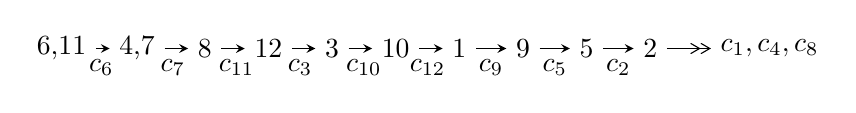
\begin{tikzpicture}[x=23pt, y=7pt]
	% node
	\node (A0) at (-1/8, 0) {6,11};
	\node (A1) at (17/16, 0) {4,7};
	\node (A2) at (17/8, 0) {8};
	\node (A3) at (25/8, 0) {12};
	\node (A4) at (33/8, 0) {3};
	\node (A5) at (41/8, 0) {10};
	\node (A6) at (49/8, 0) {1};
	\node (A7) at (57/8, 0) {9};
	\node (A8) at (65/8, 0) {5};
	\node (A9) at (73/8, 0) {2};
	\node (C1) at (1/2, -1) {$c_{6}$};
	\node (C2) at (13/8, -1) {$c_{7}$};
	\node (C3) at (21/8, -1) {$c_{11}$};
	\node (C4) at (29/8, -1) {$c_{3}$};
	\node (C5) at (37/8, -1) {$c_{10}$};
	\node (C6) at (45/8, -1) {$c_{12}$};
	\node (C7) at (53/8, -1) {$c_{9}$};
	\node (C8) at (61/8, -1) {$c_{5}$};
	\node (C9) at (69/8, -1) {$c_{2}$};
	\node (A10) at (11, 0) {$c_{1},c_{4},c_{8}$};

	% edge
	\draw[->,>=stealth]	
	(A0) edge (A1) (A1) edge (A2) (A2) edge (A3) (A3) edge (A4) (A4) edge (A5) (A5) edge (A6) (A6) edge (A7) (A7) edge (A8) (A8) edge (A9) ;
	\draw[->>,>={angle 60}]	
	(A9) edge (A10);
\end{tikzpicture} \\ 

\end{tabular} \\

\footnotetext{
The image of knot diagram is generated by the software ``\textbf{Draw programme}" developed by Andrew Bartholomew(\url{http://www.layer8.co.uk/maths/draw/index.htm\#Running-draw}), where we modified some parts for our purpose(\url{https://github.com/CATsTAILs/LinksPainter}).
}\phantom \\ \newline 
\centering \textbf{Ideals for irreducible components\footnotemark of $X_{\text{par}}$} 
 
\begin{align*}
I^u_{1}&=\langle 
- u^{109}+u^{108}+\cdots+b-2 u,\;u^{109}- u^{108}+\cdots+a+1,\;u^{111}-2 u^{110}+\cdots+2 u-1\rangle \\
I^u_{2}&=\langle 
- u^5- u^3+b- u+1,\;u^7+u^6+2 u^5+u^4+2 u^3+u^2+a+u,\;u^9+u^8+2 u^7+u^6+3 u^5+u^4+2 u^3+u-1\rangle \\
\\
\end{align*}
\raggedright * 2 irreducible components of $\dim_{\mathbb{C}}=0$, with total 120 representations.\\
\footnotetext{All coefficients of polynomials are rational numbers. But the coefficients are sometimes approximated in decimal forms when there is not enough margin.}
\newpage
\renewcommand{\arraystretch}{1}
\centering \section*{I. $I^u_{1}= \langle - u^{109}+u^{108}+\cdots+b-2 u,\;u^{109}- u^{108}+\cdots+a+1,\;u^{111}-2 u^{110}+\cdots+2 u-1 \rangle$}
\flushleft \textbf{(i) Arc colorings}\\
\begin{tabular}{m{7pt} m{180pt} m{7pt} m{180pt} }
\flushright $a_{6}=$&$\begin{pmatrix}1\\0\end{pmatrix}$ \\
\flushright $a_{11}=$&$\begin{pmatrix}0\\u\end{pmatrix}$ \\
\flushright $a_{4}=$&$\begin{pmatrix}- u^{109}+u^{108}+\cdots+4 u^3-1\\u^{109}- u^{108}+\cdots-2 u^2+2 u\end{pmatrix}$ \\
\flushright $a_{7}=$&$\begin{pmatrix}1\\u^2\end{pmatrix}$ \\
\flushright $a_{8}=$&$\begin{pmatrix}u^{17}+2 u^{15}+5 u^{13}+6 u^{11}+7 u^9+6 u^7+4 u^5+2 u^3+u\\- u^{17}-3 u^{15}-7 u^{13}-10 u^{11}-11 u^9-8 u^7-4 u^5+u\end{pmatrix}$ \\
\flushright $a_{12}=$&$\begin{pmatrix}- u\\u\end{pmatrix}$ \\
\flushright $a_{3}=$&$\begin{pmatrix}u^{109}- u^{108}+\cdots+u-2\\u^{109}- u^{108}+\cdots+3 u^3+u\end{pmatrix}$ \\
\flushright $a_{10}=$&$\begin{pmatrix}- u^3\\u^3+u\end{pmatrix}$ \\
\flushright $a_{1}=$&$\begin{pmatrix}- u^5- u\\u^5+u^3+u\end{pmatrix}$ \\
\flushright $a_{9}=$&$\begin{pmatrix}u^5+u\\u^7+u^5+2 u^3+u\end{pmatrix}$ \\
\flushright $a_{5}=$&$\begin{pmatrix}- u^{12}- u^{10}-3 u^8-2 u^6-2 u^4- u^2+1\\- u^{14}-2 u^{12}-5 u^{10}-6 u^8-6 u^6-4 u^4- u^2\end{pmatrix}$ \\
\flushright $a_{2}=$&$\begin{pmatrix}u^{107}- u^{106}+\cdots+u-1\\u^{109}- u^{108}+\cdots-2 u^2+2 u\end{pmatrix}$\\&\end{tabular}
\flushleft \textbf{(ii) Obstruction class $= -1$}\\~\\
\flushleft \textbf{(iii) Cusp Shapes $= -4 u^{110}-2 u^{109}+\cdots-8 u-6$}\\~\\
\newpage\renewcommand{\arraystretch}{1}
\flushleft \textbf{(iv) u-Polynomials at the component}\newline \\
\begin{tabular}{m{50pt}|m{274pt}}
Crossings & \hspace{64pt}u-Polynomials at each crossing \\
\hline $$\begin{aligned}c_{1}\end{aligned}$$&$\begin{aligned}
&u^{111}+52 u^{110}+\cdots+26 u+1
\end{aligned}$\\
\hline $$\begin{aligned}c_{2},c_{4}\end{aligned}$$&$\begin{aligned}
&u^{111}-10 u^{110}+\cdots-6 u+1
\end{aligned}$\\
\hline $$\begin{aligned}c_{3},c_{7}\end{aligned}$$&$\begin{aligned}
&u^{111}+u^{110}+\cdots+1024 u+512
\end{aligned}$\\
\hline $$\begin{aligned}c_{5}\end{aligned}$$&$\begin{aligned}
&u^{111}+2 u^{110}+\cdots+71974 u+7769
\end{aligned}$\\
\hline $$\begin{aligned}c_{6},c_{11}\end{aligned}$$&$\begin{aligned}
&u^{111}+2 u^{110}+\cdots+2 u+1
\end{aligned}$\\
\hline $$\begin{aligned}c_{8}\end{aligned}$$&$\begin{aligned}
&u^{111}-8 u^{110}+\cdots-4116076 u+591991
\end{aligned}$\\
\hline $$\begin{aligned}c_{9}\end{aligned}$$&$\begin{aligned}
&u^{111}-10 u^{110}+\cdots-688 u+64
\end{aligned}$\\
\hline $$\begin{aligned}c_{10},c_{12}\end{aligned}$$&$\begin{aligned}
&u^{111}-36 u^{110}+\cdots+6 u+1
\end{aligned}$\\
\hline
\end{tabular}\\~\\
\newpage\renewcommand{\arraystretch}{1}
\flushleft \textbf{(v) Riley Polynomials at the component}\newline \\
\begin{tabular}{m{50pt}|m{274pt}}
Crossings & \hspace{64pt}Riley Polynomials at each crossing \\
\hline $$\begin{aligned}c_{1}\end{aligned}$$&$\begin{aligned}
&y^{111}+24 y^{110}+\cdots+326 y-1
\end{aligned}$\\
\hline $$\begin{aligned}c_{2},c_{4}\end{aligned}$$&$\begin{aligned}
&y^{111}-52 y^{110}+\cdots+26 y-1
\end{aligned}$\\
\hline $$\begin{aligned}c_{3},c_{7}\end{aligned}$$&$\begin{aligned}
&y^{111}+57 y^{110}+\cdots-6291456 y-262144
\end{aligned}$\\
\hline $$\begin{aligned}c_{5}\end{aligned}$$&$\begin{aligned}
&y^{111}-28 y^{110}+\cdots+4384850918 y-60357361
\end{aligned}$\\
\hline $$\begin{aligned}c_{6},c_{11}\end{aligned}$$&$\begin{aligned}
&y^{111}+36 y^{110}+\cdots+6 y-1
\end{aligned}$\\
\hline $$\begin{aligned}c_{8}\end{aligned}$$&$\begin{aligned}
&y^{111}+32 y^{110}+\cdots-6104529362122 y-350453344081
\end{aligned}$\\
\hline $$\begin{aligned}c_{9}\end{aligned}$$&$\begin{aligned}
&y^{111}+4 y^{110}+\cdots-290688 y-4096
\end{aligned}$\\
\hline $$\begin{aligned}c_{10},c_{12}\end{aligned}$$&$\begin{aligned}
&y^{111}+80 y^{110}+\cdots+34 y-1
\end{aligned}$\\
\hline
\end{tabular}\\~\\
\newpage\flushleft \textbf{(vi) Complex Volumes and Cusp Shapes}
$$\begin{array}{c|c|c}  
\text{Solutions to }I^u_{1}& \I (\text{vol} + \sqrt{-1}CS) & \text{Cusp shape}\\
 \hline 
\begin{aligned}
u &= \phantom{-}0.192632 + 0.990436 I \\
a &= \phantom{-}1.008050 - 0.604735 I \\
b &= -0.482149 + 0.126128 I\end{aligned}
 & \phantom{-}0.929563 - 0.936585 I & \phantom{-0.000000 } 0 \\ \hline\begin{aligned}
u &= \phantom{-}0.192632 - 0.990436 I \\
a &= \phantom{-}1.008050 + 0.604735 I \\
b &= -0.482149 - 0.126128 I\end{aligned}
 & \phantom{-}0.929563 + 0.936585 I & \phantom{-0.000000 } 0 \\ \hline\begin{aligned}
u &= \phantom{-}0.768909 + 0.662619 I \\
a &= -0.240296 - 0.802359 I \\
b &= \phantom{-}0.66998 - 1.65382 I\end{aligned}
 & \phantom{-}2.38224 + 2.26869 I & \phantom{-0.000000 } 0 \\ \hline\begin{aligned}
u &= \phantom{-}0.768909 - 0.662619 I \\
a &= -0.240296 + 0.802359 I \\
b &= \phantom{-}0.66998 + 1.65382 I\end{aligned}
 & \phantom{-}2.38224 - 2.26869 I & \phantom{-0.000000 } 0 \\ \hline\begin{aligned}
u &= \phantom{-}0.736461 + 0.649245 I \\
a &= -0.073525 + 0.729912 I \\
b &= -0.323443 + 1.257520 I\end{aligned}
 & \phantom{-}1.40760 - 3.27569 I & \phantom{-0.000000 } 0 \\ \hline\begin{aligned}
u &= \phantom{-}0.736461 - 0.649245 I \\
a &= -0.073525 - 0.729912 I \\
b &= -0.323443 - 1.257520 I\end{aligned}
 & \phantom{-}1.40760 + 3.27569 I & \phantom{-0.000000 } 0 \\ \hline\begin{aligned}
u &= \phantom{-}0.099843 + 1.021210 I \\
a &= -1.23478 - 0.86398 I \\
b &= \phantom{-}0.494409 + 0.608915 I\end{aligned}
 & \phantom{-}3.03959 - 1.31482 I & \phantom{-0.000000 } 0 \\ \hline\begin{aligned}
u &= \phantom{-}0.099843 - 1.021210 I \\
a &= -1.23478 + 0.86398 I \\
b &= \phantom{-}0.494409 - 0.608915 I\end{aligned}
 & \phantom{-}3.03959 + 1.31482 I & \phantom{-0.000000 } 0 \\ \hline\begin{aligned}
u &= -0.125044 + 1.022840 I \\
a &= -1.03086 - 3.37868 I \\
b &= \phantom{-}0.43919 + 2.85055 I\end{aligned}
 & \phantom{-}1.10607 + 3.24001 I & \phantom{-0.000000 } 0 \\ \hline\begin{aligned}
u &= -0.125044 - 1.022840 I \\
a &= -1.03086 + 3.37868 I \\
b &= \phantom{-}0.43919 - 2.85055 I\end{aligned}
 & \phantom{-}1.10607 - 3.24001 I & \phantom{-0.000000 } 0\\
 \hline 
 \end{array}$$\newpage$$\begin{array}{c|c|c}  
\text{Solutions to }I^u_{1}& \I (\text{vol} + \sqrt{-1}CS) & \text{Cusp shape}\\
 \hline 
\begin{aligned}
u &= \phantom{-}0.254566 + 0.926058 I \\
a &= -0.663304 + 1.129570 I \\
b &= \phantom{-}0.355086 - 0.268387 I\end{aligned}
 & \phantom{-}0.41586 - 4.48947 I & \phantom{-0.000000 } 0 \\ \hline\begin{aligned}
u &= \phantom{-}0.254566 - 0.926058 I \\
a &= -0.663304 - 1.129570 I \\
b &= \phantom{-}0.355086 + 0.268387 I\end{aligned}
 & \phantom{-}0.41586 + 4.48947 I & \phantom{-0.000000 } 0 \\ \hline\begin{aligned}
u &= \phantom{-}0.132035 + 1.037550 I \\
a &= \phantom{-}1.54187 + 0.38063 I \\
b &= -0.697523 - 0.360085 I\end{aligned}
 & \phantom{-}2.17831 - 5.68318 I & \phantom{-0.000000 } 0 \\ \hline\begin{aligned}
u &= \phantom{-}0.132035 - 1.037550 I \\
a &= \phantom{-}1.54187 - 0.38063 I \\
b &= -0.697523 + 0.360085 I\end{aligned}
 & \phantom{-}2.17831 + 5.68318 I & \phantom{-0.000000 } 0 \\ \hline\begin{aligned}
u &= -0.780211 + 0.699337 I \\
a &= -0.629537 + 0.324564 I \\
b &= \phantom{-}1.213950 + 0.649893 I\end{aligned}
 & -2.92578 - 1.14947 I & \phantom{-0.000000 } 0 \\ \hline\begin{aligned}
u &= -0.780211 - 0.699337 I \\
a &= -0.629537 - 0.324564 I \\
b &= \phantom{-}1.213950 - 0.649893 I\end{aligned}
 & -2.92578 + 1.14947 I & \phantom{-0.000000 } 0 \\ \hline\begin{aligned}
u &= \phantom{-}0.530855 + 0.908540 I \\
a &= \phantom{-}0.283621 + 0.961919 I \\
b &= -0.0916763 + 0.0351119 I\end{aligned}
 & \phantom{-}0.0533926 - 0.0055215 I & \phantom{-0.000000 } 0 \\ \hline\begin{aligned}
u &= \phantom{-}0.530855 - 0.908540 I \\
a &= \phantom{-}0.283621 - 0.961919 I \\
b &= -0.0916763 - 0.0351119 I\end{aligned}
 & \phantom{-}0.0533926 + 0.0055215 I & \phantom{-0.000000 } 0 \\ \hline\begin{aligned}
u &= -0.059280 + 1.051760 I \\
a &= -1.04895 - 2.98448 I \\
b &= \phantom{-}0.33302 + 2.14606 I\end{aligned}
 & \phantom{-}7.04699 - 3.67038 I & \phantom{-0.000000 } 0 \\ \hline\begin{aligned}
u &= -0.059280 - 1.051760 I \\
a &= -1.04895 + 2.98448 I \\
b &= \phantom{-}0.33302 - 2.14606 I\end{aligned}
 & \phantom{-}7.04699 + 3.67038 I & \phantom{-0.000000 } 0\\
 \hline 
 \end{array}$$\newpage$$\begin{array}{c|c|c}  
\text{Solutions to }I^u_{1}& \I (\text{vol} + \sqrt{-1}CS) & \text{Cusp shape}\\
 \hline 
\begin{aligned}
u &= -0.474575 + 0.941264 I \\
a &= \phantom{-}0.75085 + 1.50277 I \\
b &= \phantom{-}1.44748 - 0.42754 I\end{aligned}
 & \phantom{-}3.04019 - 5.75313 I & \phantom{-0.000000 } 0 \\ \hline\begin{aligned}
u &= -0.474575 - 0.941264 I \\
a &= \phantom{-}0.75085 - 1.50277 I \\
b &= \phantom{-}1.44748 + 0.42754 I\end{aligned}
 & \phantom{-}3.04019 + 5.75313 I & \phantom{-0.000000 } 0 \\ \hline\begin{aligned}
u &= -0.082911 + 1.051710 I \\
a &= \phantom{-}0.97495 + 3.16678 I \\
b &= -0.33502 - 2.34474 I\end{aligned}
 & \phantom{-}8.29038 + 2.01687 I & \phantom{-0.000000 } 0 \\ \hline\begin{aligned}
u &= -0.082911 - 1.051710 I \\
a &= \phantom{-}0.97495 - 3.16678 I \\
b &= -0.33502 + 2.34474 I\end{aligned}
 & \phantom{-}8.29038 - 2.01687 I & \phantom{-0.000000 } 0 \\ \hline\begin{aligned}
u &= \phantom{-}0.811413 + 0.683140 I \\
a &= -1.085650 - 0.723933 I \\
b &= \phantom{-}1.08660 - 2.57993 I\end{aligned}
 & \phantom{-}0.67183 + 6.15549 I & \phantom{-0.000000 } 0 \\ \hline\begin{aligned}
u &= \phantom{-}0.811413 - 0.683140 I \\
a &= -1.085650 + 0.723933 I \\
b &= \phantom{-}1.08660 + 2.57993 I\end{aligned}
 & \phantom{-}0.67183 - 6.15549 I & \phantom{-0.000000 } 0 \\ \hline\begin{aligned}
u &= \phantom{-}0.797576 + 0.700033 I \\
a &= \phantom{-}1.10758 + 1.37941 I \\
b &= -1.70256 + 2.35602 I\end{aligned}
 & -5.10535 + 3.01862 I & \phantom{-0.000000 } 0 \\ \hline\begin{aligned}
u &= \phantom{-}0.797576 - 0.700033 I \\
a &= \phantom{-}1.10758 - 1.37941 I \\
b &= -1.70256 - 2.35602 I\end{aligned}
 & -5.10535 - 3.01862 I & \phantom{-0.000000 } 0 \\ \hline\begin{aligned}
u &= -0.805066 + 0.693292 I \\
a &= \phantom{-}0.597661 - 0.490927 I \\
b &= -1.49235 - 0.31506 I\end{aligned}
 & -4.14766 - 5.56202 I & \phantom{-0.000000 } 0 \\ \hline\begin{aligned}
u &= -0.805066 - 0.693292 I \\
a &= \phantom{-}0.597661 + 0.490927 I \\
b &= -1.49235 + 0.31506 I\end{aligned}
 & -4.14766 + 5.56202 I & \phantom{-0.000000 } 0\\
 \hline 
 \end{array}$$\newpage$$\begin{array}{c|c|c}  
\text{Solutions to }I^u_{1}& \I (\text{vol} + \sqrt{-1}CS) & \text{Cusp shape}\\
 \hline 
\begin{aligned}
u &= -0.132451 + 1.054970 I \\
a &= \phantom{-}0.90434 + 3.23113 I \\
b &= -0.53870 - 2.53237 I\end{aligned}
 & \phantom{-}7.07789 + 6.12746 I & \phantom{-0.000000 } 0 \\ \hline\begin{aligned}
u &= -0.132451 - 1.054970 I \\
a &= \phantom{-}0.90434 - 3.23113 I \\
b &= -0.53870 + 2.53237 I\end{aligned}
 & \phantom{-}7.07789 - 6.12746 I & \phantom{-0.000000 } 0 \\ \hline\begin{aligned}
u &= -0.146614 + 1.057970 I \\
a &= -0.83912 - 3.15269 I \\
b &= \phantom{-}0.59773 + 2.48167 I\end{aligned}
 & \phantom{-}4.91151 + 11.83360 I & \phantom{-0.000000 } 0 \\ \hline\begin{aligned}
u &= -0.146614 - 1.057970 I \\
a &= -0.83912 + 3.15269 I \\
b &= \phantom{-}0.59773 - 2.48167 I\end{aligned}
 & \phantom{-}4.91151 - 11.83360 I & \phantom{-0.000000 } 0 \\ \hline\begin{aligned}
u &= \phantom{-}0.096016 + 0.926261 I \\
a &= -0.046350 - 1.080040 I \\
b &= -0.233565 + 0.499204 I\end{aligned}
 & \phantom{-}1.90349 - 1.53560 I & \phantom{-0.000000 } 0 \\ \hline\begin{aligned}
u &= \phantom{-}0.096016 - 0.926261 I \\
a &= -0.046350 + 1.080040 I \\
b &= -0.233565 - 0.499204 I\end{aligned}
 & \phantom{-}1.90349 + 1.53560 I & \phantom{-0.000000 } 0 \\ \hline\begin{aligned}
u &= -0.764877 + 0.747204 I \\
a &= -0.782753 - 0.110036 I \\
b &= \phantom{-}0.560754 + 1.224240 I\end{aligned}
 & -3.69681 - 0.59851 I & \phantom{-0.000000 } 0 \\ \hline\begin{aligned}
u &= -0.764877 - 0.747204 I \\
a &= -0.782753 + 0.110036 I \\
b &= \phantom{-}0.560754 - 1.224240 I\end{aligned}
 & -3.69681 + 0.59851 I & \phantom{-0.000000 } 0 \\ \hline\begin{aligned}
u &= -0.568939 + 0.906736 I \\
a &= \phantom{-}0.47634 + 2.73143 I \\
b &= \phantom{-}2.65902 - 1.01527 I\end{aligned}
 & -1.20931 + 2.19749 I & \phantom{-0.000000 } 0 \\ \hline\begin{aligned}
u &= -0.568939 - 0.906736 I \\
a &= \phantom{-}0.47634 - 2.73143 I \\
b &= \phantom{-}2.65902 + 1.01527 I\end{aligned}
 & -1.20931 - 2.19749 I & \phantom{-0.000000 } 0\\
 \hline 
 \end{array}$$\newpage$$\begin{array}{c|c|c}  
\text{Solutions to }I^u_{1}& \I (\text{vol} + \sqrt{-1}CS) & \text{Cusp shape}\\
 \hline 
\begin{aligned}
u &= \phantom{-}0.820991 + 0.687464 I \\
a &= \phantom{-}1.30100 + 0.59172 I \\
b &= -1.08489 + 2.81057 I\end{aligned}
 & -1.63250 + 11.81960 I & \phantom{-0.000000 } 0 \\ \hline\begin{aligned}
u &= \phantom{-}0.820991 - 0.687464 I \\
a &= \phantom{-}1.30100 - 0.59172 I \\
b &= -1.08489 - 2.81057 I\end{aligned}
 & -1.63250 - 11.81960 I & \phantom{-0.000000 } 0 \\ \hline\begin{aligned}
u &= -0.507517 + 0.943536 I \\
a &= -0.81181 - 1.85142 I \\
b &= -1.63254 + 0.69181 I\end{aligned}
 & \phantom{-}4.96384 - 0.11752 I & \phantom{-0.000000 } 0 \\ \hline\begin{aligned}
u &= -0.507517 - 0.943536 I \\
a &= -0.81181 + 1.85142 I \\
b &= -1.63254 - 0.69181 I\end{aligned}
 & \phantom{-}4.96384 + 0.11752 I & \phantom{-0.000000 } 0 \\ \hline\begin{aligned}
u &= \phantom{-}0.772006 + 0.772780 I \\
a &= \phantom{-}1.58909 - 0.90180 I \\
b &= \phantom{-}0.576947 + 1.122740 I\end{aligned}
 & -6.36063 - 0.71203 I & \phantom{-0.000000 } 0 \\ \hline\begin{aligned}
u &= \phantom{-}0.772006 - 0.772780 I \\
a &= \phantom{-}1.58909 + 0.90180 I \\
b &= \phantom{-}0.576947 - 1.122740 I\end{aligned}
 & -6.36063 + 0.71203 I & \phantom{-0.000000 } 0 \\ \hline\begin{aligned}
u &= \phantom{-}0.662337 + 0.870835 I \\
a &= -0.397275 + 0.149125 I \\
b &= -0.0950051 + 0.0447575 I\end{aligned}
 & -1.01013 - 2.56602 I & \phantom{-0.000000 } 0 \\ \hline\begin{aligned}
u &= \phantom{-}0.662337 - 0.870835 I \\
a &= -0.397275 - 0.149125 I \\
b &= -0.0950051 - 0.0447575 I\end{aligned}
 & -1.01013 + 2.56602 I & \phantom{-0.000000 } 0 \\ \hline\begin{aligned}
u &= -0.815391 + 0.729941 I \\
a &= \phantom{-}0.142260 - 0.616883 I \\
b &= -1.009020 + 0.511024 I\end{aligned}
 & -5.63875 - 0.21059 I & \phantom{-0.000000 } 0 \\ \hline\begin{aligned}
u &= -0.815391 - 0.729941 I \\
a &= \phantom{-}0.142260 + 0.616883 I \\
b &= -1.009020 - 0.511024 I\end{aligned}
 & -5.63875 + 0.21059 I & \phantom{-0.000000 } 0\\
 \hline 
 \end{array}$$\newpage$$\begin{array}{c|c|c}  
\text{Solutions to }I^u_{1}& \I (\text{vol} + \sqrt{-1}CS) & \text{Cusp shape}\\
 \hline 
\begin{aligned}
u &= -0.770455 + 0.789444 I \\
a &= \phantom{-}1.106370 + 0.534564 I \\
b &= -0.27456 - 1.87357 I\end{aligned}
 & -5.82240 + 3.12989 I & \phantom{-0.000000 } 0 \\ \hline\begin{aligned}
u &= -0.770455 - 0.789444 I \\
a &= \phantom{-}1.106370 - 0.534564 I \\
b &= -0.27456 + 1.87357 I\end{aligned}
 & -5.82240 - 3.12989 I & \phantom{-0.000000 } 0 \\ \hline\begin{aligned}
u &= \phantom{-}0.581600 + 0.937909 I \\
a &= -0.659104 - 0.661539 I \\
b &= \phantom{-}0.100577 - 0.196830 I\end{aligned}
 & \phantom{-}0.34882 - 4.22670 I & \phantom{-0.000000 } 0 \\ \hline\begin{aligned}
u &= \phantom{-}0.581600 - 0.937909 I \\
a &= -0.659104 + 0.661539 I \\
b &= \phantom{-}0.100577 + 0.196830 I\end{aligned}
 & \phantom{-}0.34882 + 4.22670 I & \phantom{-0.000000 } 0 \\ \hline\begin{aligned}
u &= -0.808577 + 0.760102 I \\
a &= \phantom{-}0.420874 + 0.731250 I \\
b &= \phantom{-}0.507807 - 1.307110 I\end{aligned}
 & -6.15982 - 3.10465 I & \phantom{-0.000000 } 0 \\ \hline\begin{aligned}
u &= -0.808577 - 0.760102 I \\
a &= \phantom{-}0.420874 - 0.731250 I \\
b &= \phantom{-}0.507807 + 1.307110 I\end{aligned}
 & -6.15982 + 3.10465 I & \phantom{-0.000000 } 0 \\ \hline\begin{aligned}
u &= \phantom{-}0.767617 + 0.814930 I \\
a &= -1.341450 + 0.226399 I \\
b &= \phantom{-}0.254417 - 0.631786 I\end{aligned}
 & -1.58344 - 3.65437 I & \phantom{-0.000000 } 0 \\ \hline\begin{aligned}
u &= \phantom{-}0.767617 - 0.814930 I \\
a &= -1.341450 - 0.226399 I \\
b &= \phantom{-}0.254417 + 0.631786 I\end{aligned}
 & -1.58344 + 3.65437 I & \phantom{-0.000000 } 0 \\ \hline\begin{aligned}
u &= -0.573335 + 0.970305 I \\
a &= -1.17424 - 2.43459 I \\
b &= -1.72069 + 1.50758 I\end{aligned}
 & \phantom{-}5.43993 + 3.94383 I & \phantom{-0.000000 } 0 \\ \hline\begin{aligned}
u &= -0.573335 - 0.970305 I \\
a &= -1.17424 + 2.43459 I \\
b &= -1.72069 - 1.50758 I\end{aligned}
 & \phantom{-}5.43993 - 3.94383 I & \phantom{-0.000000 } 0\\
 \hline 
 \end{array}$$\newpage$$\begin{array}{c|c|c}  
\text{Solutions to }I^u_{1}& \I (\text{vol} + \sqrt{-1}CS) & \text{Cusp shape}\\
 \hline 
\begin{aligned}
u &= \phantom{-}0.789834 + 0.812667 I \\
a &= \phantom{-}1.64616 - 0.11664 I \\
b &= -0.543734 + 0.979094 I\end{aligned}
 & -3.81432 - 8.80179 I & \phantom{-0.000000 } 0 \\ \hline\begin{aligned}
u &= \phantom{-}0.789834 - 0.812667 I \\
a &= \phantom{-}1.64616 + 0.11664 I \\
b &= -0.543734 - 0.979094 I\end{aligned}
 & -3.81432 + 8.80179 I & \phantom{-0.000000 } 0 \\ \hline\begin{aligned}
u &= -0.592860 + 0.980993 I \\
a &= \phantom{-}1.24435 + 2.51142 I \\
b &= \phantom{-}1.64111 - 1.71076 I\end{aligned}
 & \phantom{-}3.89569 + 9.64082 I & \phantom{-0.000000 } 0 \\ \hline\begin{aligned}
u &= -0.592860 - 0.980993 I \\
a &= \phantom{-}1.24435 - 2.51142 I \\
b &= \phantom{-}1.64111 + 1.71076 I\end{aligned}
 & \phantom{-}3.89569 - 9.64082 I & \phantom{-0.000000 } 0 \\ \hline\begin{aligned}
u &= \phantom{-}0.734585 + 0.916006 I \\
a &= -0.239524 - 0.207158 I \\
b &= -0.060534 + 0.753628 I\end{aligned}
 & -1.26885 - 2.02626 I & \phantom{-0.000000 } 0 \\ \hline\begin{aligned}
u &= \phantom{-}0.734585 - 0.916006 I \\
a &= -0.239524 + 0.207158 I \\
b &= -0.060534 - 0.753628 I\end{aligned}
 & -1.26885 + 2.02626 I & \phantom{-0.000000 } 0 \\ \hline\begin{aligned}
u &= -0.729555 + 0.940810 I \\
a &= -1.65103 - 0.88700 I \\
b &= \phantom{-}0.22575 + 2.04696 I\end{aligned}
 & -5.35605 + 2.54553 I & \phantom{-0.000000 } 0 \\ \hline\begin{aligned}
u &= -0.729555 - 0.940810 I \\
a &= -1.65103 + 0.88700 I \\
b &= \phantom{-}0.22575 - 2.04696 I\end{aligned}
 & -5.35605 - 2.54553 I & \phantom{-0.000000 } 0 \\ \hline\begin{aligned}
u &= -0.080571 + 0.801768 I \\
a &= -0.68517 + 1.41490 I \\
b &= \phantom{-}1.165590 - 0.301891 I\end{aligned}
 & -0.875710 + 0.948469 I & -8.68611 + 0. I\phantom{ +0.000000I} \\ \hline\begin{aligned}
u &= -0.080571 - 0.801768 I \\
a &= -0.68517 - 1.41490 I \\
b &= \phantom{-}1.165590 + 0.301891 I\end{aligned}
 & -0.875710 - 0.948469 I & -8.68611 + 0. I\phantom{ +0.000000I}\\
 \hline 
 \end{array}$$\newpage$$\begin{array}{c|c|c}  
\text{Solutions to }I^u_{1}& \I (\text{vol} + \sqrt{-1}CS) & \text{Cusp shape}\\
 \hline 
\begin{aligned}
u &= \phantom{-}0.754108 + 0.928714 I \\
a &= \phantom{-}0.020894 + 0.559672 I \\
b &= -0.170032 - 1.257680 I\end{aligned}
 & -3.45583 + 2.99333 I & \phantom{-0.000000 } 0 \\ \hline\begin{aligned}
u &= \phantom{-}0.754108 - 0.928714 I \\
a &= \phantom{-}0.020894 - 0.559672 I \\
b &= -0.170032 + 1.257680 I\end{aligned}
 & -3.45583 - 2.99333 I & \phantom{-0.000000 } 0 \\ \hline\begin{aligned}
u &= \phantom{-}0.726683 + 0.953612 I \\
a &= -0.404649 - 0.333661 I \\
b &= \phantom{-}1.15069 - 1.19096 I\end{aligned}
 & -5.80570 - 4.95975 I & \phantom{-0.000000 } 0 \\ \hline\begin{aligned}
u &= \phantom{-}0.726683 - 0.953612 I \\
a &= -0.404649 + 0.333661 I \\
b &= \phantom{-}1.15069 + 1.19096 I\end{aligned}
 & -5.80570 + 4.95975 I & \phantom{-0.000000 } 0 \\ \hline\begin{aligned}
u &= -0.716470 + 0.968399 I \\
a &= \phantom{-}1.009940 + 0.983135 I \\
b &= \phantom{-}0.24035 - 1.43149 I\end{aligned}
 & -3.02213 + 6.21900 I & \phantom{-0.000000 } 0 \\ \hline\begin{aligned}
u &= -0.716470 - 0.968399 I \\
a &= \phantom{-}1.009940 - 0.983135 I \\
b &= \phantom{-}0.24035 + 1.43149 I\end{aligned}
 & -3.02213 - 6.21900 I & \phantom{-0.000000 } 0 \\ \hline\begin{aligned}
u &= \phantom{-}0.682596 + 1.003720 I \\
a &= -1.72286 + 0.90870 I \\
b &= -0.69420 - 1.57701 I\end{aligned}
 & \phantom{-}2.44885 - 2.15395 I & \phantom{-0.000000 } 0 \\ \hline\begin{aligned}
u &= \phantom{-}0.682596 - 1.003720 I \\
a &= -1.72286 - 0.90870 I \\
b &= -0.69420 + 1.57701 I\end{aligned}
 & \phantom{-}2.44885 + 2.15395 I & \phantom{-0.000000 } 0 \\ \hline\begin{aligned}
u &= -0.710907 + 0.998558 I \\
a &= \phantom{-}0.08358 + 1.50967 I \\
b &= \phantom{-}1.13414 - 0.92782 I\end{aligned}
 & -2.02005 + 6.79446 I & \phantom{-0.000000 } 0 \\ \hline\begin{aligned}
u &= -0.710907 - 0.998558 I \\
a &= \phantom{-}0.08358 - 1.50967 I \\
b &= \phantom{-}1.13414 + 0.92782 I\end{aligned}
 & -2.02005 - 6.79446 I & \phantom{-0.000000 } 0\\
 \hline 
 \end{array}$$\newpage$$\begin{array}{c|c|c}  
\text{Solutions to }I^u_{1}& \I (\text{vol} + \sqrt{-1}CS) & \text{Cusp shape}\\
 \hline 
\begin{aligned}
u &= \phantom{-}0.696196 + 1.008940 I \\
a &= \phantom{-}1.91104 - 1.30509 I \\
b &= \phantom{-}0.92895 + 2.06413 I\end{aligned}
 & \phantom{-}3.41635 - 7.82906 I & \phantom{-0.000000 } 0 \\ \hline\begin{aligned}
u &= \phantom{-}0.696196 - 1.008940 I \\
a &= \phantom{-}1.91104 + 1.30509 I \\
b &= \phantom{-}0.92895 - 2.06413 I\end{aligned}
 & \phantom{-}3.41635 + 7.82906 I & \phantom{-0.000000 } 0 \\ \hline\begin{aligned}
u &= -0.746068 + 0.973664 I \\
a &= -1.42525 - 0.12220 I \\
b &= \phantom{-}0.82226 + 1.25984 I\end{aligned}
 & -5.50452 + 8.94364 I & \phantom{-0.000000 } 0 \\ \hline\begin{aligned}
u &= -0.746068 - 0.973664 I \\
a &= -1.42525 + 0.12220 I \\
b &= \phantom{-}0.82226 - 1.25984 I\end{aligned}
 & -5.50452 - 8.94364 I & \phantom{-0.000000 } 0 \\ \hline\begin{aligned}
u &= \phantom{-}0.718823 + 1.003060 I \\
a &= -2.07659 + 2.17491 I \\
b &= -1.80915 - 3.12071 I\end{aligned}
 & -4.18525 - 8.73612 I & \phantom{-0.000000 } 0 \\ \hline\begin{aligned}
u &= \phantom{-}0.718823 - 1.003060 I \\
a &= -2.07659 - 2.17491 I \\
b &= -1.80915 + 3.12071 I\end{aligned}
 & -4.18525 + 8.73612 I & \phantom{-0.000000 } 0 \\ \hline\begin{aligned}
u &= -0.738208 + 0.993906 I \\
a &= \phantom{-}0.927077 - 0.659401 I \\
b &= -1.101950 - 0.318264 I\end{aligned}
 & -4.83099 + 6.04293 I & \phantom{-0.000000 } 0 \\ \hline\begin{aligned}
u &= -0.738208 - 0.993906 I \\
a &= \phantom{-}0.927077 + 0.659401 I \\
b &= -1.101950 + 0.318264 I\end{aligned}
 & -4.83099 - 6.04293 I & \phantom{-0.000000 } 0 \\ \hline\begin{aligned}
u &= -0.720095 + 1.008540 I \\
a &= \phantom{-}0.41204 - 1.59057 I \\
b &= -1.45541 + 0.62359 I\end{aligned}
 & -3.19045 + 11.30350 I & \phantom{-0.000000 } 0 \\ \hline\begin{aligned}
u &= -0.720095 - 1.008540 I \\
a &= \phantom{-}0.41204 + 1.59057 I \\
b &= -1.45541 - 0.62359 I\end{aligned}
 & -3.19045 - 11.30350 I & \phantom{-0.000000 } 0\\
 \hline 
 \end{array}$$\newpage$$\begin{array}{c|c|c}  
\text{Solutions to }I^u_{1}& \I (\text{vol} + \sqrt{-1}CS) & \text{Cusp shape}\\
 \hline 
\begin{aligned}
u &= \phantom{-}0.719408 + 1.015160 I \\
a &= \phantom{-}2.36088 - 1.88696 I \\
b &= \phantom{-}1.04853 + 3.16425 I\end{aligned}
 & \phantom{-}1.67951 - 11.91070 I & \phantom{-0.000000 } 0 \\ \hline\begin{aligned}
u &= \phantom{-}0.719408 - 1.015160 I \\
a &= \phantom{-}2.36088 + 1.88696 I \\
b &= \phantom{-}1.04853 - 3.16425 I\end{aligned}
 & \phantom{-}1.67951 + 11.91070 I & \phantom{-0.000000 } 0 \\ \hline\begin{aligned}
u &= \phantom{-}0.725093 + 1.016800 I \\
a &= -2.46825 + 1.95770 I \\
b &= -0.94944 - 3.40309 I\end{aligned}
 & -0.6299 - 17.6207 I & \phantom{-0.000000 } 0 \\ \hline\begin{aligned}
u &= \phantom{-}0.725093 - 1.016800 I \\
a &= -2.46825 - 1.95770 I \\
b &= -0.94944 + 3.40309 I\end{aligned}
 & -0.6299 + 17.6207 I & \phantom{-0.000000 } 0 \\ \hline\begin{aligned}
u &= -0.574352 + 0.418607 I \\
a &= \phantom{-}0.135427 + 0.714012 I \\
b &= \phantom{-}0.86196 + 1.26612 I\end{aligned}
 & \phantom{-}2.54612 - 5.10023 I & -7.16882 + 3.19715 I \\ \hline\begin{aligned}
u &= -0.574352 - 0.418607 I \\
a &= \phantom{-}0.135427 - 0.714012 I \\
b &= \phantom{-}0.86196 - 1.26612 I\end{aligned}
 & \phantom{-}2.54612 + 5.10023 I & -7.16882 - 3.19715 I \\ \hline\begin{aligned}
u &= -0.631566 + 0.179431 I \\
a &= \phantom{-}1.55073 + 0.65579 I \\
b &= \phantom{-}0.078384 + 1.100650 I\end{aligned}
 & \phantom{-}0.93401 + 9.47471 I & -10.17613 - 7.65520 I \\ \hline\begin{aligned}
u &= -0.631566 - 0.179431 I \\
a &= \phantom{-}1.55073 - 0.65579 I \\
b &= \phantom{-}0.078384 - 1.100650 I\end{aligned}
 & \phantom{-}0.93401 - 9.47471 I & -10.17613 + 7.65520 I \\ \hline\begin{aligned}
u &= -0.560215 + 0.341895 I \\
a &= -0.456081 - 0.838719 I \\
b &= -0.630414 - 1.220460 I\end{aligned}
 & \phantom{-}3.99504 + 0.35322 I & -5.03327 - 2.38344 I \\ \hline\begin{aligned}
u &= -0.560215 - 0.341895 I \\
a &= -0.456081 + 0.838719 I \\
b &= -0.630414 + 1.220460 I\end{aligned}
 & \phantom{-}3.99504 - 0.35322 I & -5.03327 + 2.38344 I\\
 \hline 
 \end{array}$$\newpage$$\begin{array}{c|c|c}  
\text{Solutions to }I^u_{1}& \I (\text{vol} + \sqrt{-1}CS) & \text{Cusp shape}\\
 \hline 
\begin{aligned}
u &= -0.607988 + 0.205302 I \\
a &= -1.32956 - 0.79282 I \\
b &= -0.205681 - 1.140070 I\end{aligned}
 & \phantom{-}3.06262 + 3.92490 I & -6.94599 - 3.74176 I \\ \hline\begin{aligned}
u &= -0.607988 - 0.205302 I \\
a &= -1.32956 + 0.79282 I \\
b &= -0.205681 + 1.140070 I\end{aligned}
 & \phantom{-}3.06262 - 3.92490 I & -6.94599 + 3.74176 I \\ \hline\begin{aligned}
u &= \phantom{-}0.606436 + 0.043814 I \\
a &= \phantom{-}0.197367 - 0.784558 I \\
b &= -0.207695 + 0.574254 I\end{aligned}
 & -2.33432 + 1.63935 I & -11.54858 - 4.00697 I \\ \hline\begin{aligned}
u &= \phantom{-}0.606436 - 0.043814 I \\
a &= \phantom{-}0.197367 + 0.784558 I \\
b &= -0.207695 - 0.574254 I\end{aligned}
 & -2.33432 - 1.63935 I & -11.54858 + 4.00697 I \\ \hline\begin{aligned}
u &= \phantom{-}0.570119 + 0.177210 I \\
a &= \phantom{-}0.626226 - 0.746167 I \\
b &= -0.639347 + 0.300541 I\end{aligned}
 & -1.64918 - 3.56067 I & -12.02219 + 5.47193 I \\ \hline\begin{aligned}
u &= \phantom{-}0.570119 - 0.177210 I \\
a &= \phantom{-}0.626226 + 0.746167 I \\
b &= -0.639347 - 0.300541 I\end{aligned}
 & -1.64918 + 3.56067 I & -12.02219 - 5.47193 I \\ \hline\begin{aligned}
u &= -0.525944 + 0.152741 I \\
a &= \phantom{-}1.48425 + 1.60870 I \\
b &= \phantom{-}0.338855 + 0.955316 I\end{aligned}
 & -2.56426 + 1.24826 I & -11.02453 - 5.32858 I \\ \hline\begin{aligned}
u &= -0.525944 - 0.152741 I \\
a &= \phantom{-}1.48425 - 1.60870 I \\
b &= \phantom{-}0.338855 - 0.955316 I\end{aligned}
 & -2.56426 - 1.24826 I & -11.02453 + 5.32858 I \\ \hline\begin{aligned}
u &= \phantom{-}0.413113 + 0.265236 I \\
a &= -0.828742 + 0.732041 I \\
b &= \phantom{-}0.558168 + 0.007894 I\end{aligned}
 & -0.745453 + 0.267249 I & -9.83522 + 0.75496 I \\ \hline\begin{aligned}
u &= \phantom{-}0.413113 - 0.265236 I \\
a &= -0.828742 - 0.732041 I \\
b &= \phantom{-}0.558168 - 0.007894 I\end{aligned}
 & -0.745453 - 0.267249 I & -9.83522 - 0.75496 I\\
 \hline 
 \end{array}$$\newpage$$\begin{array}{c|c|c}  
\text{Solutions to }I^u_{1}& \I (\text{vol} + \sqrt{-1}CS) & \text{Cusp shape}\\
 \hline 
\begin{aligned}
u &= \phantom{-}0.376387\phantom{ +0.000000I} \\
a &= -0.936204\phantom{ +0.000000I} \\
b &= \phantom{-}0.379146\phantom{ +0.000000I}\end{aligned}
 & -0.758702\phantom{ +0.000000I} & -12.9630\phantom{ +0.000000I}\\
 \hline 
 \end{array}$$\newpage\newpage\renewcommand{\arraystretch}{1}
\centering \section*{II. $I^u_{2}= \langle - u^5- u^3+b- u+1,\;u^7+u^6+2 u^5+u^4+2 u^3+u^2+a+u,\;u^9+u^8+2 u^7+u^6+3 u^5+u^4+2 u^3+u-1 \rangle$}
\flushleft \textbf{(i) Arc colorings}\\
\begin{tabular}{m{7pt} m{180pt} m{7pt} m{180pt} }
\flushright $a_{6}=$&$\begin{pmatrix}1\\0\end{pmatrix}$ \\
\flushright $a_{11}=$&$\begin{pmatrix}0\\u\end{pmatrix}$ \\
\flushright $a_{4}=$&$\begin{pmatrix}- u^7- u^6-2 u^5- u^4-2 u^3- u^2- u\\u^5+u^3+u-1\end{pmatrix}$ \\
\flushright $a_{7}=$&$\begin{pmatrix}1\\u^2\end{pmatrix}$ \\
\flushright $a_{8}=$&$\begin{pmatrix}1\\u^2\end{pmatrix}$ \\
\flushright $a_{12}=$&$\begin{pmatrix}- u\\u\end{pmatrix}$ \\
\flushright $a_{3}=$&$\begin{pmatrix}- u^7- u^6-2 u^5- u^4-2 u^3- u^2- u\\u^5+u^3+u-1\end{pmatrix}$ \\
\flushright $a_{10}=$&$\begin{pmatrix}- u^3\\u^3+u\end{pmatrix}$ \\
\flushright $a_{1}=$&$\begin{pmatrix}- u^5- u\\u^5+u^3+u\end{pmatrix}$ \\
\flushright $a_{9}=$&$\begin{pmatrix}u^5+u\\u^7+u^5+2 u^3+u\end{pmatrix}$ \\
\flushright $a_{5}=$&$\begin{pmatrix}u^5+u\\- u^5- u^3- u\end{pmatrix}$ \\
\flushright $a_{2}=$&$\begin{pmatrix}- u^7- u^6-3 u^5- u^4-2 u^3- u^2-2 u\\2 u^5+2 u^3+2 u-1\end{pmatrix}$\\&\end{tabular}
\flushleft \textbf{(ii) Obstruction class $= 1$}\\~\\
\flushleft \textbf{(iii) Cusp Shapes $= -4 u^7-4 u^6-3 u^5-3 u^4-6 u^3-3 u^2+u-13$}\\~\\
\newpage\renewcommand{\arraystretch}{1}
\flushleft \textbf{(iv) u-Polynomials at the component}\newline \\
\begin{tabular}{m{50pt}|m{274pt}}
Crossings & \hspace{64pt}u-Polynomials at each crossing \\
\hline $$\begin{aligned}c_{1},c_{2}\end{aligned}$$&$\begin{aligned}
&(u-1)^9
\end{aligned}$\\
\hline $$\begin{aligned}c_{3},c_{7}\end{aligned}$$&$\begin{aligned}
&u^9
\end{aligned}$\\
\hline $$\begin{aligned}c_{4}\end{aligned}$$&$\begin{aligned}
&(u+1)^9
\end{aligned}$\\
\hline $$\begin{aligned}c_{5},c_{8}\end{aligned}$$&$\begin{aligned}
&u^9+u^8-2 u^7-3 u^6+u^5+3 u^4+2 u^3- u-1
\end{aligned}$\\
\hline $$\begin{aligned}c_{6}\end{aligned}$$&$\begin{aligned}
&u^9+u^8+2 u^7+u^6+3 u^5+u^4+2 u^3+u-1
\end{aligned}$\\
\hline $$\begin{aligned}c_{9}\end{aligned}$$&$\begin{aligned}
&u^9+5 u^8+12 u^7+15 u^6+9 u^5- u^4-4 u^3-2 u^2+u+1
\end{aligned}$\\
\hline $$\begin{aligned}c_{10}\end{aligned}$$&$\begin{aligned}
&u^9+3 u^8+8 u^7+13 u^6+17 u^5+17 u^4+12 u^3+6 u^2+u-1
\end{aligned}$\\
\hline $$\begin{aligned}c_{11}\end{aligned}$$&$\begin{aligned}
&u^9- u^8+2 u^7- u^6+3 u^5- u^4+2 u^3+u+1
\end{aligned}$\\
\hline $$\begin{aligned}c_{12}\end{aligned}$$&$\begin{aligned}
&u^9-3 u^8+8 u^7-13 u^6+17 u^5-17 u^4+12 u^3-6 u^2+u+1
\end{aligned}$\\
\hline
\end{tabular}\\~\\
\newpage\renewcommand{\arraystretch}{1}
\flushleft \textbf{(v) Riley Polynomials at the component}\newline \\
\begin{tabular}{m{50pt}|m{274pt}}
Crossings & \hspace{64pt}Riley Polynomials at each crossing \\
\hline $$\begin{aligned}c_{1},c_{2},c_{4}\end{aligned}$$&$\begin{aligned}
&(y-1)^9
\end{aligned}$\\
\hline $$\begin{aligned}c_{3},c_{7}\end{aligned}$$&$\begin{aligned}
&y^9
\end{aligned}$\\
\hline $$\begin{aligned}c_{5},c_{8}\end{aligned}$$&$\begin{aligned}
&y^9-5 y^8+12 y^7-15 y^6+9 y^5+y^4-4 y^3+2 y^2+y-1
\end{aligned}$\\
\hline $$\begin{aligned}c_{6},c_{11}\end{aligned}$$&$\begin{aligned}
&y^9+3 y^8+8 y^7+13 y^6+17 y^5+17 y^4+12 y^3+6 y^2+y-1
\end{aligned}$\\
\hline $$\begin{aligned}c_{9}\end{aligned}$$&$\begin{aligned}
&y^9- y^8+12 y^7-7 y^6+37 y^5+y^4-10 y^2+5 y-1
\end{aligned}$\\
\hline $$\begin{aligned}c_{10},c_{12}\end{aligned}$$&$\begin{aligned}
&y^9+7 y^8+20 y^7+25 y^6+5 y^5-15 y^4+22 y^2+13 y-1
\end{aligned}$\\
\hline
\end{tabular}\\~\\
\newpage\flushleft \textbf{(vi) Complex Volumes and Cusp Shapes}
$$\begin{array}{c|c|c}  
\text{Solutions to }I^u_{2}& \I (\text{vol} + \sqrt{-1}CS) & \text{Cusp shape}\\
 \hline 
\begin{aligned}
u &= \phantom{-}0.140343 + 0.966856 I \\
a &= \phantom{-}0.900982 - 0.594909 I \\
b &= -0.663053 + 0.788921 I\end{aligned}
 & \phantom{-}0.13850 - 2.09337 I & -6.69021 + 3.87975 I \\ \hline\begin{aligned}
u &= \phantom{-}0.140343 - 0.966856 I \\
a &= \phantom{-}0.900982 + 0.594909 I \\
b &= -0.663053 - 0.788921 I\end{aligned}
 & \phantom{-}0.13850 + 2.09337 I & -6.69021 - 3.87975 I \\ \hline\begin{aligned}
u &= \phantom{-}0.628449 + 0.875112 I \\
a &= \phantom{-}0.249476 + 1.304240 I \\
b &= -1.52709 - 0.20930 I\end{aligned}
 & -2.26187 - 2.45442 I & -12.49381 + 3.35442 I \\ \hline\begin{aligned}
u &= \phantom{-}0.628449 - 0.875112 I \\
a &= \phantom{-}0.249476 - 1.304240 I \\
b &= -1.52709 + 0.20930 I\end{aligned}
 & -2.26187 + 2.45442 I & -12.49381 - 3.35442 I \\ \hline\begin{aligned}
u &= -0.796005 + 0.733148 I \\
a &= -0.766570 + 0.255687 I \\
b &= \phantom{-}0.224752 + 0.919301 I\end{aligned}
 & -6.01628 - 1.33617 I & -13.53709 + 1.22905 I \\ \hline\begin{aligned}
u &= -0.796005 - 0.733148 I \\
a &= -0.766570 - 0.255687 I \\
b &= \phantom{-}0.224752 - 0.919301 I\end{aligned}
 & -6.01628 + 1.33617 I & -13.53709 - 1.22905 I \\ \hline\begin{aligned}
u &= -0.728966 + 0.986295 I \\
a &= \phantom{-}0.721488 + 0.307914 I \\
b &= \phantom{-}0.124310 - 1.173370 I\end{aligned}
 & -5.24306 + 7.08493 I & -12.02676 - 6.64241 I \\ \hline\begin{aligned}
u &= -0.728966 - 0.986295 I \\
a &= \phantom{-}0.721488 - 0.307914 I \\
b &= \phantom{-}0.124310 + 1.173370 I\end{aligned}
 & -5.24306 - 7.08493 I & -12.02676 + 6.64241 I \\ \hline\begin{aligned}
u &= \phantom{-}0.512358\phantom{ +0.000000I} \\
a &= -1.21075\phantom{ +0.000000I} \\
b &= -0.317835\phantom{ +0.000000I}\end{aligned}
 & -2.84338\phantom{ +0.000000I} & -14.5040\phantom{ +0.000000I}\\
 \hline 
 \end{array}$$\newpage
\newpage\renewcommand{\arraystretch}{1}
\centering \section*{ III. u-Polynomials}
\begin{tabular}{m{50pt}|m{274pt}}
Crossings & \hspace{64pt}u-Polynomials at each crossing \\
\hline $$\begin{aligned}c_{1}\end{aligned}$$&$\begin{aligned}
&((u-1)^9)(u^{111}+52 u^{110}+\cdots+26 u+1)
\end{aligned}$\\
\hline $$\begin{aligned}c_{2}\end{aligned}$$&$\begin{aligned}
&((u-1)^9)(u^{111}-10 u^{110}+\cdots-6 u+1)
\end{aligned}$\\
\hline $$\begin{aligned}c_{3},c_{7}\end{aligned}$$&$\begin{aligned}
&u^9(u^{111}+u^{110}+\cdots+1024 u+512)
\end{aligned}$\\
\hline $$\begin{aligned}c_{4}\end{aligned}$$&$\begin{aligned}
&((u+1)^9)(u^{111}-10 u^{110}+\cdots-6 u+1)
\end{aligned}$\\
\hline $$\begin{aligned}c_{5}\end{aligned}$$&$\begin{aligned}
&(u^9+u^8-2 u^7-3 u^6+u^5+3 u^4+2 u^3- u-1)\\
&\cdot(u^{111}+2 u^{110}+\cdots+71974 u+7769)
\end{aligned}$\\
\hline $$\begin{aligned}c_{6}\end{aligned}$$&$\begin{aligned}
&(u^9+u^8+\cdots+u-1)(u^{111}+2 u^{110}+\cdots+2 u+1)
\end{aligned}$\\
\hline $$\begin{aligned}c_{8}\end{aligned}$$&$\begin{aligned}
&(u^9+u^8-2 u^7-3 u^6+u^5+3 u^4+2 u^3- u-1)\\
&\cdot(u^{111}-8 u^{110}+\cdots-4116076 u+591991)
\end{aligned}$\\
\hline $$\begin{aligned}c_{9}\end{aligned}$$&$\begin{aligned}
&(u^9+5 u^8+12 u^7+15 u^6+9 u^5- u^4-4 u^3-2 u^2+u+1)\\
&\cdot(u^{111}-10 u^{110}+\cdots-688 u+64)
\end{aligned}$\\
\hline $$\begin{aligned}c_{10}\end{aligned}$$&$\begin{aligned}
&(u^9+3 u^8+8 u^7+13 u^6+17 u^5+17 u^4+12 u^3+6 u^2+u-1)\\
&\cdot(u^{111}-36 u^{110}+\cdots+6 u+1)
\end{aligned}$\\
\hline $$\begin{aligned}c_{11}\end{aligned}$$&$\begin{aligned}
&(u^9- u^8+\cdots+u+1)(u^{111}+2 u^{110}+\cdots+2 u+1)
\end{aligned}$\\
\hline $$\begin{aligned}c_{12}\end{aligned}$$&$\begin{aligned}
&(u^9-3 u^8+8 u^7-13 u^6+17 u^5-17 u^4+12 u^3-6 u^2+u+1)\\
&\cdot(u^{111}-36 u^{110}+\cdots+6 u+1)
\end{aligned}$\\
\hline
\end{tabular}\newpage\renewcommand{\arraystretch}{1}
\centering \section*{ IV. Riley Polynomials}
\begin{tabular}{m{50pt}|m{274pt}}
Crossings & \hspace{64pt}Riley Polynomials at each crossing \\
\hline $$\begin{aligned}c_{1}\end{aligned}$$&$\begin{aligned}
&((y-1)^9)(y^{111}+24 y^{110}+\cdots+326 y-1)
\end{aligned}$\\
\hline $$\begin{aligned}c_{2},c_{4}\end{aligned}$$&$\begin{aligned}
&((y-1)^9)(y^{111}-52 y^{110}+\cdots+26 y-1)
\end{aligned}$\\
\hline $$\begin{aligned}c_{3},c_{7}\end{aligned}$$&$\begin{aligned}
&y^9(y^{111}+57 y^{110}+\cdots-6291456 y-262144)
\end{aligned}$\\
\hline $$\begin{aligned}c_{5}\end{aligned}$$&$\begin{aligned}
&(y^9-5 y^8+12 y^7-15 y^6+9 y^5+y^4-4 y^3+2 y^2+y-1)\\
&\cdot(y^{111}-28 y^{110}+\cdots+4384850918 y-60357361)
\end{aligned}$\\
\hline $$\begin{aligned}c_{6},c_{11}\end{aligned}$$&$\begin{aligned}
&(y^9+3 y^8+8 y^7+13 y^6+17 y^5+17 y^4+12 y^3+6 y^2+y-1)\\
&\cdot(y^{111}+36 y^{110}+\cdots+6 y-1)
\end{aligned}$\\
\hline $$\begin{aligned}c_{8}\end{aligned}$$&$\begin{aligned}
&(y^9-5 y^8+12 y^7-15 y^6+9 y^5+y^4-4 y^3+2 y^2+y-1)\\
&\cdot(y^{111}+32 y^{110}+\cdots-6104529362122 y-350453344081)
\end{aligned}$\\
\hline $$\begin{aligned}c_{9}\end{aligned}$$&$\begin{aligned}
&(y^9- y^8+12 y^7-7 y^6+37 y^5+y^4-10 y^2+5 y-1)\\
&\cdot(y^{111}+4 y^{110}+\cdots-290688 y-4096)
\end{aligned}$\\
\hline $$\begin{aligned}c_{10},c_{12}\end{aligned}$$&$\begin{aligned}
&(y^9+7 y^8+20 y^7+25 y^6+5 y^5-15 y^4+22 y^2+13 y-1)\\
&\cdot(y^{111}+80 y^{110}+\cdots+34 y-1)
\end{aligned}$\\
\hline
\end{tabular}
\vskip 2pc
\end{document}